
\begin{figure}[!htbp]
\begin{center}
	%
	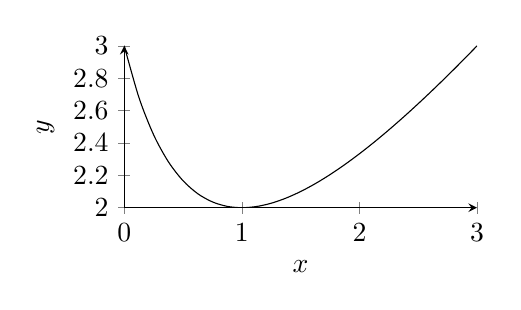
\begin{tikzpicture}
	[
		xscale	= 1,	% to scale horizontally everything but the text
		yscale	= 1,	% to scale vertically everything but the text
		declare function = {f(\x) = 0.5 * \x^2;},
	]
		%
		\begin{axis}
		[
			xmode					= linear,
			ymode					= linear,
			width					= 0.5\columnwidth,
			height					= 0.3\columnwidth,
			axis x line				= bottom,	% bottom | middle | top
			axis y line				= left,		% left | middle | right
			xlabel					= {$x$},
			ylabel					= {$y$},
		]
			%
			\addplot
			[
				no marks,
				smooth,
				domain	= 0:3
			]
			{(x^2 + 3)/(x + 1)};
			%
			% ALLOWED OPERATORS
			% +, -, *, /, abs, round, floor, mod, <, >, max, min, sin, cos, tan,
			% deg (conversion from radians to degrees),
			% rad (conversion from degrees to radians),
			% atan, asin, acos, cot, sec, cosec, exp, ln,
			% sqrt, the constants pi and e, ^ (power operation), factorial,
			% rand (random between −1 and 1), rnd (random between 0 and 1),
			% number format conversions hex, Hex, oct, bin
			%
		\end{axis}
		%
	\end{tikzpicture}
	\end{center}
	%
\caption{function xxx}
\label{fig:xxx}
\end{figure}
